\section{The phonon-assisted amplitude}\label{sec:13.2}

At the onset of \cref{we:13-onset} a particle of \SI{0.3374}{MeV} transfers $q^* = \SI{0.90}{keV}$ along a valley axis of silicon and deposits \SI{1.185}{eV}. The final state has a hole at the valence-band maximum, an electron at the bottom of a conduction valley, \SI{1.94}{keV} away in crystal momentum, and a transverse acoustic phonon of \SI{14.8}{meV} that carries the remaining \SI{1.0}{keV}. Neither the density coupling nor the electron--phonon coupling reaches this final state alone. The density $n_e(\vect{q})$ creates pairs of crystal momentum $\vect{q}$, and at $q = \SI{0.90}{keV}$ the cheapest of them costs about \SI{1.9}{eV} (\cref{fig:13-window}). The electron--phonon coupling creates a phonon and can change the crystal momentum of an electron by any amount, but it cannot lift an electron across a gap of \SI{1.17}{eV} with the tens of meV that a phonon brings. The amplitude is therefore of second order, with one density vertex and one electron--phonon vertex.

\subsection{Final states and the second-order amplitude}

The target is the crystal at the base point of \cref{sec:8.5} with one coupling added: independent electrons in Bloch states $\psi_{n\vect{k}}$ with energies $\varepsilon_{n\vect{k}}$ (Kohn--Sham energies with the conduction bands raised by the scissor shift, as in \cref{sec:10.1}), harmonic phonons $(\vect{Q},\nu)$ with energies $\omega_{\vect{Q}\nu}$, and the electron--phonon Hamiltonian $H_{\mathrm{ep}}$ of \cref{eq:A.6-Hep}, linear in the displacements, with the screened vertex $g_{mn\nu}(\vect{k},\vect{Q})$ of \cref{eq:A.6-g}. The dark matter couples to the electron density, through the row of \cref{eq:8.2-spectrum} with $\mathfrak{D}_{ee} = |\tilde V(\vect{q})|^2$. The target enters only through the matrix elements of $n_e(\vect{q})$ (\cref{eq:3.2-ne}) that appear in the structure factor \cref{eq:4.2-Sab}. In the zero-phonon response of \cref{sec:10.1}, the matrix element of $n_e(\vect{q})$ is the density vertex $\rho_{cv}(\vect{k},\vect{q})$ of \cref{eq:3.2-rho}. In the phonon-assisted response a second-order amplitude replaces the density vertex.

The initial state $|i\rangle$ has the valence bands filled, the conduction bands empty and $n_{\vect{Q}\nu}$ phonons in each mode. A one-phonon final state has an electron in $(c,\vect{k}')$, a hole in $(v,\vect{k})$ and the phonon occupations of $|i\rangle$ changed in one mode,
\begin{equation}
  |f\rangle = c^\dagger_{c\vect{k}'}c_{v\vect{k}}\,|i'\rangle , \qquad
  \vect{k}' = \vect{k} + \vect{q} + \vect{Q} , \qquad
  E_f - E_i = \varepsilon_{c\vect{k}'} - \varepsilon_{v\vect{k}} \pm \omega_{\vect{Q}\nu} ,
  \label{eq:13.2-final}
\end{equation}
where $|i'\rangle$ has one phonon more in $(-\vect{Q},\nu)$ (upper sign, emission) or one fewer in $(\vect{Q},\nu)$ (lower sign, absorption), as in \cref{eq:A.6-weights}, and $\vect{k}'$ is folded back into the zone. The momentum transfer $\vect{q}$ is not folded: the density vertex keeps it whole and carries the Umklapp vector in its plane wave (\cref{eq:3.2-rho}). Conservation of crystal momentum leaves the phonon whatever crystal momentum the pair needs beyond $\vect{q}$: $\vect{Q} = \vect{k}' - \vect{k} - \vect{q}$ modulo a reciprocal-lattice vector, as in \cref{sec:13.1}. The density vertex and the electron--phonon vertex are both diagonal in spin, so the electron and the hole have the same spin, and the spin sum enters only the rate (\cref{sec:13.3}). With spin--orbit coupling the bands are spinors, and the formulas below hold with the band indices running over spinor bands.

The second-order amplitude follows from \cref{eq:2.4-c2} as for light (\cref{sec:6.5}). The dark matter gives up the energy $\omega$ and the momentum $\vect{q}$ at its own vertex, and its kinetic energy cancels from every denominator. In the ordering in which the density vertex acts first, the intermediate state $|m\rangle$ already holds the energy $\omega$; in the ordering in which the electron--phonon vertex acts first, the intermediate state does not:
\begin{equation}
  \langle f|n_e^{(2)}(\vect{q})|i\rangle = \sum_m\left[\frac{\langle f|H_{\mathrm{ep}}|m\rangle\langle m|n_e(\vect{q})|i\rangle}{E_i + \omega - E_m} + \frac{\langle f|n_e(\vect{q})|m\rangle\langle m|H_{\mathrm{ep}}|i\rangle}{E_i - E_m}\right] , \qquad
  \omega = E_f - E_i .
  \label{eq:13.2-T}
\end{equation}
This matrix element takes the place of $\langle f|n_e(\vect{q})|i\rangle$ in \cref{eq:4.2-Sab}. The condition $\omega = E_f - E_i$ is the energy delta function of the structure factor, and the amplitude is needed only there, on the energy shell. The sum runs over many-electron states with their phonons, and it is finite as long as no $E_m$ equals $E_i + \omega$ or $E_i$. An $E_m$ equal to $E_i$ never occurs in an insulator. An $E_m$ equal to $E_i + \omega$ would mean that the density alone creates a real zero-phonon pair at $(\vect{q},\omega)$, and no such pair exists while $\omega$ lies below $E_{\mathrm{min}}(\vect{q})$ (\cref{eq:13.2-doff}).

\subsection{Four paths}

Both vertices are one-body operators, $n_e(\vect{q}) = \sum\rho_{mn}c^\dagger c$ and $H_{\mathrm{ep}} = N^{-1/2}\sum g_{mn\nu}c^\dagger c\,B_{\vect{Q}\nu}$, and each moves one electron. Acting first on the filled valence bands, a vertex can only move an electron from a filled state into an empty one, so every intermediate state $|m\rangle$ holds exactly one electron--hole pair. (A term that moves an electron back into the state it came from needs a momentum transfer equal to a reciprocal-lattice vector, $\vect{q} = \vect{G}$ or $\vect{Q} = 0$. It has measure zero in the integrals over $\vect{q}$ and $\vect{Q}$, and \cref{app:D.35} shows that even there it adds nothing new.) The second vertex must turn that intermediate pair into the final pair $(c\vect{k}';\,v\vect{k})$, again by moving one electron. The second vertex can do so in two ways. It can move the intermediate electron into $(c,\vect{k}')$, if the intermediate hole is already the final one, $(v,\vect{k})$; or it can move the electron of $(v,\vect{k})$ into the intermediate hole, if the intermediate electron is already the final one, $(c,\vect{k}')$. The two ways, combined with the two orderings of the vertices, make four paths:
\begin{equation}
  \begin{aligned}
  \text{A:}&\quad \frac{g_{cp\nu}(\vect{k}+\vect{q},\vect{Q})\,\rho_{pv}(\vect{k},\vect{q})}{\omega - \varepsilon_{p,\vect{k}+\vect{q}} + \varepsilon_{v\vect{k}}} ,
  &\text{B:}&\quad \frac{\rho_{cp}(\vect{k}+\vect{Q},\vect{q})\,g_{pv\nu}(\vect{k},\vect{Q})}{\varepsilon_{v\vect{k}} - \varepsilon_{p,\vect{k}+\vect{Q}} \mp \omega_{\vect{Q}\nu}} , &&\quad p\ \text{empty}, \\
  \text{C:}&\quad -\frac{\rho_{cp}(\vect{k}+\vect{Q},\vect{q})\,g_{pv\nu}(\vect{k},\vect{Q})}{\omega - \varepsilon_{c\vect{k}'} + \varepsilon_{p,\vect{k}+\vect{Q}}} ,
  &\text{D:}&\quad -\frac{g_{cp\nu}(\vect{k}+\vect{q},\vect{Q})\,\rho_{pv}(\vect{k},\vect{q})}{\varepsilon_{p,\vect{k}+\vect{q}} - \varepsilon_{c\vect{k}'} \mp \omega_{\vect{Q}\nu}} , &&\quad p\ \text{filled}.
  \end{aligned}
  \label{eq:13.2-paths}
\end{equation}
Each term is the contribution of one intermediate band $p$, with the common factor $N^{-1/2}(n_{\vect{Q}\nu} + \frac12 \pm \frac12)^{1/2}$ of the phonon vertex taken out. \Cref{fig:13-paths} draws the four paths as time-ordered diagrams.

\begin{figure}[tbp]
  \centering
  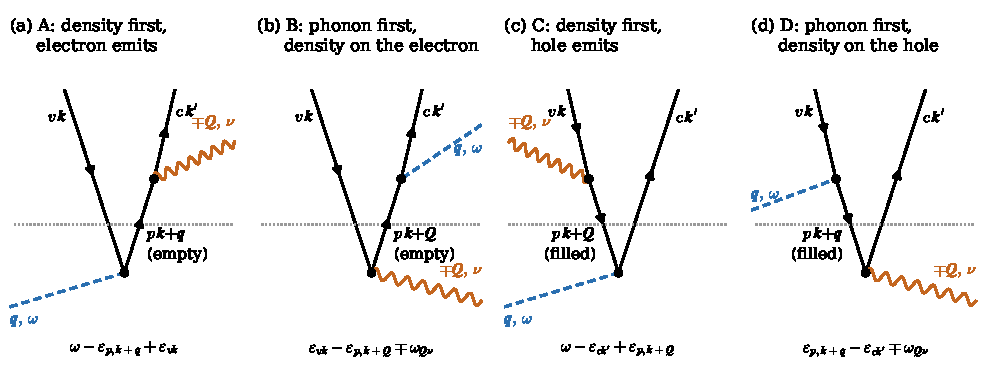
\includegraphics[width=\linewidth]{figures/ch13/fig13_2.pdf}
  \caption{The four paths of the phonon-assisted electron-recoil amplitude, \cref{eq:13.2-paths}, as time-ordered diagrams. Time runs upward. Lines with upward arrows are electrons, lines with downward arrows are holes; the dashed line is the dark-matter density vertex, which delivers momentum $\vect{q}$ and energy $\omega$; the wavy line is the phonon, emitted with $-\vect{Q}$ or absorbed with $+\vect{Q}$. The dotted line cuts the intermediate state, whose energy denominator is printed below each panel. Every path ends in the same final state, an electron in $(c,\vect{k}')$ with $\vect{k}' = \vect{k} + \vect{q} + \vect{Q}$ and a hole in $(v,\vect{k})$. (a)--(d)~Paths A to D, with an electron in an empty band $p$ between the vertices in A and B and a hole in a filled band $p$ in C and D. Schematic; no line length or angle carries a number.}
  \label{fig:13-paths}
\end{figure}

In paths A and B an electron propagates between the vertices. In A the density creates a pair, $(p,\vect{k}+\vect{q})$ with $(v,\vect{k})$, and the electron then scatters into $(c,\vect{k}')$ by emitting or absorbing the phonon; the pair created in A is the virtual zero-phonon pair of \cref{sec:10.1}, carried to the final state by the phonon. In B the phonon vertex creates a virtual pair at crystal momentum $\vect{Q}$, $(p,\vect{k}+\vect{Q})$ with $(v,\vect{k})$, and the density then scatters the electron by $\vect{q}$. The intermediate band $p$ must be empty in both A and B, since an electron cannot enter a filled state. In paths C and D a hole propagates. In C the density creates the final electron from a filled state $(p,\vect{k}+\vect{Q})$, and the phonon vertex then moves an electron from $(v,\vect{k})$ into the hole that the final electron left. In D the phonon vertex creates the final electron from a filled state $(p,\vect{k}+\vect{q})$, and the density then fills the hole in $(p,\vect{k}+\vect{q})$ from $(v,\vect{k})$. The denominators contain the energies of the intermediate pairs. They also contain $\omega$ in the density-first orderings A and C, and the phonon energy in the phonon-first orderings B and D, where the phonon has already been emitted or absorbed.

The minus signs of C and D come from the order of the fermion operators. In path A the operators act as $c^\dagger_cc_p\,c^\dagger_pc_v = c^\dagger_c(1 - n_p)c_v$, which is $c^\dagger_cc_v$ on a state with $p$ empty. In path C they act as $c^\dagger_pc_v\,c^\dagger_cc_p$, and three exchanges of neighboring operators bring them into the order $-c^\dagger_c\,(c^\dagger_pc_p)\,c_v = -c^\dagger_c\,n_p\,c_v$, which is $-c^\dagger_cc_v$ on a state with $p$ filled. The same reordering gives $-1$ for D. The four paths are those of phonon-assisted absorption (\cref{sec:6.5}), with the velocity vertex of light replaced by the density vertex; summed over every band they give the two-term amplitude of phonon-assisted absorption~\cites[Eq.~(200)]{giustino2017electron}[Eqs.~(2) and~(3)]{noffsinger2012phonon}. Replacing the velocity vertex by the density vertex changes the crystal momenta at which the intermediate states sit: the photon-first intermediate state of \cref{eq:6.5-M} sits at the crystal momentum of the hole, and the density-first intermediate state of path A at $\vect{k}+\vect{q}$.

\subsection{The unrestricted band sum}

On the energy shell the hole paths change form. Insert $\omega = \varepsilon_{c\vect{k}'} - \varepsilon_{v\vect{k}} \pm \omega_{\vect{Q}\nu}$ of \cref{eq:13.2-final} into their denominators. The denominator of C becomes $\varepsilon_{p,\vect{k}+\vect{Q}} - \varepsilon_{v\vect{k}} \pm \omega_{\vect{Q}\nu}$, and with its minus sign, path C becomes the expression of path B for a filled band $p$. The denominator of D becomes $\varepsilon_{p,\vect{k}+\vect{q}} - \varepsilon_{v\vect{k}} - \omega$, and path D becomes the expression of path A for a filled band. A single electron could not take paths A and B through a filled band: Pauli blocking forbids them. In the many-electron amplitude the blocked paths return as exchange partners, paths C and D, with exactly the one-electron value. In path C the electron that ends in $(c,\vect{k}')$ comes from the filled band $p$, and the electron from $(v,\vect{k})$ takes its place; exchanging the two identical electrons turns path C into path B with the electron from $v$ passing through $p$. The fermion sign of the exchange and the sign of the hole denominator cancel, and the four paths combine into the amplitude of one electron alone in the bands:
\begin{keyresult}[Phonon-assisted amplitude]
On the energy shell, the second-order amplitude \cref{eq:13.2-T} into the final state \cref{eq:13.2-final} is
\begin{equation}
  \begin{gathered}
  \langle f|n_e^{(2)}(\vect{q})|i\rangle = \frac{1}{\sqrt N}\bigl(n_{\vect{Q}\nu} + \tfrac12 \pm \tfrac12\bigr)^{1/2}M^{\pm}_{cv\nu}(\vect{k},\vect{q},\vect{Q}) , \\
  M^{\pm}_{cv\nu}(\vect{k},\vect{q},\vect{Q}) = \sum_p\left[\frac{g_{cp\nu}(\vect{k}+\vect{q},\vect{Q})\,\rho_{pv}(\vect{k},\vect{q})}{\omega - \varepsilon_{p,\vect{k}+\vect{q}} + \varepsilon_{v\vect{k}}} + \frac{\rho_{cp}(\vect{k}+\vect{Q},\vect{q})\,g_{pv\nu}(\vect{k},\vect{Q})}{\varepsilon_{v\vect{k}} - \varepsilon_{p,\vect{k}+\vect{Q}} \mp \omega_{\vect{Q}\nu}}\right] ,
  \end{gathered}
  \label{eq:13.2-M}
\end{equation}
with $\omega = \varepsilon_{c\vect{k}'} - \varepsilon_{v\vect{k}} \pm \omega_{\vect{Q}\nu}$, the upper sign for emission, and the sum over every band $p$, filled or empty, including $p = v$ and $p = c$.
\end{keyresult}
\noindent The amplitude $M^\pm$ is dimensionless, like $\rho$, and of order one in $N$; the factor $N^{-1/2}$ is that of \cref{eq:A.6-Hep}, and it is removed by the independent sum over $\vect{Q}$ in the rate (\cref{sec:13.3}). In operator form, $M^\pm$ is the matrix element between $(v,\vect{k})$ and $(c,\vect{k}')$ of the two vertices joined by the resolvent of the one-electron Hamiltonian, with no projector on empty states. The general statement, for any two one-body vertices acting on an independent-particle ground state, is proved in \cref{app:D.35}; \cref{eq:6.5-M} is its instance for light.

The band-sum form \cref{eq:13.2-M}, an instance of the band-sum theorem of \cref{app:D.35}, holds on the energy shell only. Off the shell the denominators of C and D differ from those of the blocked electron paths by $\omega - (E_f - E_i)$. Any quantity that needs the amplitude off the shell has to keep the four paths of \cref{eq:13.2-paths} as they stand; the real part of a phonon-assisted response is an example. The band-sum form also requires independent electrons, where the intermediate and final states are single Slater determinants. With the electron--hole attraction the final pair is an exciton, and the paths are rebuilt from exciton states in \cref{sec:13.8}. Finally, the band-sum form needs every intermediate state to be off the shell, a condition that \cref{eq:13.2-doff} below guarantees inside the window.

When the intermediate states are thought of as virtual electrons, the natural truncation keeps only empty intermediate bands, and this truncation gets the amplitude wrong by a factor of order one: \cref{we:13-exchange} finds a factor of 2.4 in the rate of a model, or 1.6 with the other phase convention of its phonon vertex. The intraband terms belong to the sum as well. In path A with $p = v$, the density moves the valence electron within its band and the phonon then lifts it across the gap. In path B with $p = c$, the phonon creates the pair and the density moves the electron within the conduction band. These two terms carry the largest density vertices at small $q$, since $\rho_{vv}$ and $\rho_{cc}$ tend to one, and they cancel at $\vect{q} = 0$. At $\vect{q} = 0$, $\rho_{pv}(\vect{k},0) = \delta_{pv}$, path A reduces to $g_{cv\nu}(\vect{k},\vect{Q})/\omega$ and path B to $g_{cv\nu}(\vect{k},\vect{Q})/(\varepsilon_{v\vect{k}} - \varepsilon_{c,\vect{k}+\vect{Q}} \mp \omega_{\vect{Q}\nu}) = -g_{cv\nu}(\vect{k},\vect{Q})/\omega$, and
\begin{equation}
  M^{\pm}_{cv\nu}(\vect{k},0,\vect{Q}) = 0 .
  \label{eq:13.2-q0}
\end{equation}
The zero of \cref{eq:13.2-q0} is exact, because $n_e(0)$ is the number of electrons, which commutes with the Hamiltonian and causes no transition at any order. The amplitude therefore starts at first order in $\vect{q}$, as the zero-phonon vertex $\rho_{cv}$ does (\cref{eq:3.2-optical}), and the limit $\vect{q}\to0$ that connects the amplitude to phonon-assisted optical absorption is taken in \cref{sec:13.5}. A calculation that truncates the band sum, or treats the intraband terms with a different vertex than the interband ones, loses \cref{eq:13.2-q0} and with it the small-$q$ behavior of the rate.

\begin{workedexample}{Exchange partners in a two-band chain}\label{we:13-exchange}
The smallest system in which all four paths appear has two bands and one phonon mode. Take a chain of $N = 6$ cells with two orbitals per cell, A at $x = 0$ and B at $x = a/2$, on-site energies $+\SI{0.4}{eV}$ and $-\SI{0.4}{eV}$, and hoppings \SI{1.6}{eV} within the cell and \SI{1.0}{eV} between cells. The electrons are spinless, since the spin only doubles a rate. The density vertex is $\ee^{\ii qx}$ on the orbital positions. One dispersionless phonon of energy $\omega_{\mathrm{ph}} = \SI{60}{meV}$ shifts the two on-site energies in opposite directions. Its vertex is \SI{0.2}{eV} times the matrix element of $\sum_R\ee^{\ii QR}(n_{R\mathrm{A}} - n_{R\mathrm{B}})$ between the two Bloch states it connects, with the phase of the displacement wave taken at the origin $R$ of each cell. Crystal momenta are multiples of $2\pi/6a$, shifted by a twist of \SI{0.3}{rad} in the boundary condition around the ring (\SI{0.05}{rad} per crystal momentum). The twist lifts the degeneracy of $k$ and $-k$. The lower band is filled and the upper is empty, with the smallest gap near the zone boundary, \SI{1.448}{eV} with the twist and \SI{1.442}{eV} without it. All parameters are illustrative.

Put the final pair at the gap, $(v,k)$ and $(c,k)$, with $q = 2\times2\pi/6a$ and a phonon emitted with $Q = -q$. The energy deposited on the shell is $\omega = \SI{1.448}{eV} + \omega_{\mathrm{ph}} = \SI{1.508}{eV}$, while the cheapest zero-phonon pair at this $q$ costs $E_{\mathrm{min}}(q) = \SI{2.912}{eV}$: the zero-phonon channel is closed by a margin of \SI{1.40}{eV}. The four terms of \cref{eq:13.2-paths} are:
\begin{center}
\small
\begin{tabular}{llrr}
  \toprule
  path & intermediate pair & denominator (eV) & term \\
  \midrule
  A & electron $(c,k+q)$, hole $(v,k)$ & $-1.552$ & $+0.0176 - 0.0246\,\ii$ \\
  B & electron $(c,k+Q)$, hole $(v,k)$ & $-3.060$ & $+0.0439 + 0.0051\,\ii$ \\
  C & electron $(c,k)$, hole $(v,k+Q)$ & $-1.492$ & $+0.0062 - 0.0379\,\ii$ \\
  D & electron $(c,k)$, hole $(v,k+q)$ & $-3.120$ & $-0.0313 - 0.0354\,\ii$ \\
  \bottomrule
\end{tabular}
\end{center}
In the one-electron sum \cref{eq:13.2-M}, the blocked forms are path B with $p = v$, with denominator $\varepsilon_{v k} - \varepsilon_{v,k+Q} - \omega_{\mathrm{ph}} = +\SI{1.492}{eV}$, and path A with $p = v$, with denominator $+\SI{3.120}{eV}$. Their values are $+0.0062 - 0.0379\,\ii$ and $-0.0313 - 0.0354\,\ii$, equal to C and D to all printed digits: the hole denominators have the sign opposite to that of the blocked forms, and the fermion sign undoes the sign change. In path A with $p = v$, the intraband density vertex, $|\rho_{vv}|^2 = 0.642$, is larger than the interband one, $|\rho_{cv}|^2 = 0.358$, and the hole paths are not a small correction: $|\mathrm{C} + \mathrm{D}| = 0.077$, against $|\mathrm{A} + \mathrm{B}| = 0.065$ and $|M| = 0.100$.

The sum over the empty band alone, paths A and B, gives $+0.0615 - 0.0195\,\ii$, with $|M|^2$ at 0.42 of the correct value: a factor of 2.4 in the rate. With the phase of the displacement wave taken at the orbital positions, $\ee^{\ii Qx}$ with $Q = -q$, the coupling itself changes: then $|M| = 0.107$, and the empty band alone is off by a factor of 1.6. The size of the error depends on the model; the fact that the error is of order one does not.

Move $\omega$ off the shell by \SI{0.10}{eV}. Path A changes as its formula says, B is unchanged, and C becomes $+0.0066 - 0.0406\,\ii$ against $+0.0062 - 0.0379\,\ii$ for the blocked form. The many-body total now differs from the unrestricted one-electron sum by 3.7\%. The exchange partners are equal only where energy is conserved.
\end{workedexample}

\subsection{No interference with the zero-phonon line}

A dark-matter particle that deposits $\omega$ at $\vect{q}$ could, in principle, produce the same pair with and without a phonon, and the two amplitudes might interfere. At second order in $g$ they do not. The rate is a sum over final states of the squared total amplitude into each. The zero-phonon final states have the phonon occupations of $|i\rangle$; their amplitude is $\rho_{cv}$ at zeroth order in $g$, with corrections of order $g^2$ from a phonon emitted and reabsorbed. The final states of \cref{eq:13.2-final} have one occupation changed by one; their amplitude starts at first order. A cross term needs two amplitudes into the same final state, and states that differ in the occupation of one mode are orthogonal. Through order $g^2$, squaring therefore gives two separate rates and no term that mixes them. The zero-phonon rate is $|\rho_{cv}|^2$ plus twice the real part of $\rho_{cv}^*$ times the order-$g^2$ amplitude, and the phonon-assisted rate is $|M^\pm|^2$. A thermal initial state changes nothing, since its density matrix is diagonal in the phonon occupations and the change of occupation between initial and final state remains a good label.

The order-$g^2$ corrections to the zero-phonon amplitude therefore belong to the zero-phonon line; they are the Fan--Migdal and Allen--Heine self-energies of \cref{sec:6.3} and the virtual-phonon vertex. These corrections shift and reweight the zero-phonon line (\cref{sec:8.6,sec:13.7}), and they are never added to the phonon-assisted rate. Inside the window, $\omega < E_{\mathrm{min}}(\vect{q})$, no zero-phonon final state exists at the energy $\omega$, and the question of interference does not arise at any order. Above $E_{\mathrm{min}}(\vect{q})$ both channels are open, and the absence of interference still holds at this order. The Fano term of \cref{sec:8.6} is a different interference: inside the one-phonon final states, between the part of path A in which the zero-phonon pair is real and the paths in which it is not. It belongs to the phonon-dressed sector and, at the level of one-body self-energies, vanishes in silicon and germanium.

\subsection{The adiabatic (Herzberg--Teller) form}

The denominators of \cref{eq:13.2-M} decide both whether the amplitude is finite and how it can be computed. Each is the energy by which an intermediate pair misses the energy shell, and on the shell each is the energy of a pair minus a known amount. For $p$ empty in the first term, the pair $(p,\vect{k}+\vect{q};\,v,\vect{k})$ has crystal momentum $\vect{q}$, and the denominator is $\omega$ minus its energy. For $p$ filled in the second term, path C, the denominator is the energy of the pair $(c,\vect{k}';\,p,\vect{k}+\vect{Q})$, again of crystal momentum $\vect{q}$, minus $\omega$. Both denominators are at least $E_{\mathrm{min}}(\vect{q}) - \omega$ in size, with $E_{\mathrm{min}}$ of \cref{eq:3.3-Emin}. In the two remaining cases the intermediate pair has crystal momentum $\vect{Q}$ and costs at least $\Eg$, and the denominator differs from the pair energy by $\omega_{\vect{Q}\nu}$. The smallest off-shell distance of \cref{eq:8.5-theta} is therefore bounded below on the shell:
\begin{equation}
  \delta_{\mathrm{off}} \ge \min\bigl(E_{\mathrm{min}}(\vect{q}) - \omega,\;\Eg - \omega_{\vect{Q}\nu}\bigr) .
  \label{eq:13.2-doff}
\end{equation}
Below $E_{\mathrm{min}}(\vect{q})$ every denominator is negative or positive by a finite margin, and the amplitude needs no width, no $\ii0^+$ and no subtraction. The only denominators that can approach zero are those of the virtual zero-phonon pairs at $\vect{q}$, the electron of path A and the hole of path C. As $\omega$ approaches $E_{\mathrm{min}}(\vect{q})$, the virtual zero-phonon pairs become real pairs that emit a phonon after they are created; the process becomes a cascade, and the second-order amplitude stops being a separate quantity. \Cref{sec:13.6} turns the bound \cref{eq:13.2-doff} into the window inside which \cref{eq:13.2-M} holds. In silicon the bound for pairs at $\vect{Q}$ is at least $\SI{1.17}{eV} - \SI{64}{meV} = \SI{1.11}{eV}$, and the tighter bound is the margin below the zero-phonon edge. At the onset of \cref{we:13-onset}, where $\omega \approx \SI{1.19}{eV}$ against $E_{\mathrm{min}} \approx \SI{1.9}{eV}$, the margin is about \SI{0.7}{eV}.

The phonon energy enters the amplitude twice: in the energy balance, where it sets the threshold, and in the denominators, where it is small against $\delta_{\mathrm{off}}$. Dropping it from the denominators, with $\omega = \varepsilon_{c\vect{k}'} - \varepsilon_{v\vect{k}}$ in the first term, gives the adiabatic amplitude
\begin{equation}
  M^{\mathrm{ad}}_{cv\nu}(\vect{k},\vect{q},\vect{Q}) = \sum_p\left[\frac{g_{cp\nu}(\vect{k}+\vect{q},\vect{Q})\,\rho_{pv}(\vect{k},\vect{q})}{\varepsilon_{c\vect{k}'} - \varepsilon_{p,\vect{k}+\vect{q}}} + \frac{\rho_{cp}(\vect{k}+\vect{Q},\vect{q})\,g_{pv\nu}(\vect{k},\vect{Q})}{\varepsilon_{v\vect{k}} - \varepsilon_{p,\vect{k}+\vect{Q}}}\right] ,
  \label{eq:13.2-Mad}
\end{equation}
the same for emission and absorption, with the states degenerate with $(c,\vect{k}')$ left out of the first term and those degenerate with $(v,\vect{k})$ left out of the second. The adiabatic amplitude is a derivative of the zero-phonon vertex. Replace the phonon operator $B_{\vect{Q}\nu}$ in $H_{\mathrm{ep}}$ by a number $b$, with its conjugate for $B_{-\vect{Q}\nu}$. The electrons then feel the static potential of a frozen displacement wave of the mode, \cref{eq:A.6-u} with $B \to b$, which couples $\psi_{n\vect{k}}$ to the states at $\vect{k}\pm\vect{Q}$ with the matrix elements $N^{-1/2}b\,g_{mn\nu}(\vect{k},\vect{Q})$ and their conjugates. By first-order perturbation theory, the valence state $\psi_{v\vect{k}}$ acquires the admixture $N^{-1/2}b\sum_p\psi_{p,\vect{k}+\vect{Q}}\,g_{pv\nu}(\vect{k},\vect{Q})/(\varepsilon_{v\vect{k}} - \varepsilon_{p,\vect{k}+\vect{Q}})$, and the conduction state $\psi_{c\vect{k}'}$ acquires states at $\vect{k}'-\vect{Q} = \vect{k}+\vect{q}$ through the conjugate coupling. The terms with $b^*$ reach crystal momenta $\vect{k}\pm2\vect{Q}$ away from the pair and drop out unless $2\vect{Q}$ is a reciprocal-lattice vector. The transition density $\rho_{cv}(\vect{k},\vect{q}) = \langle\psi_{c\vect{k}'}|\ee^{\ii\vect{q}\cdot\vect{r}}|\psi_{v\vect{k}}\rangle$ vanishes in the perfect lattice, because $\vect{k}' \ne \vect{k}+\vect{q}$, and becomes nonzero at first order in $b$. The change of the conduction state gives the first term of \cref{eq:13.2-Mad} and the change of the valence state the second, and
\begin{equation}
  \frac{\partial\rho_{cv}}{\partial b} = \frac{1}{\sqrt N}\,M^{\mathrm{ad}}_{cv\nu}(\vect{k},\vect{q},\vect{Q}) , \qquad
  \langle f|n_e^{(2)}(\vect{q})|i\rangle \simeq \langle n'|B_{\vect{Q}\nu}|n\rangle\,\frac{\partial\rho_{cv}}{\partial b} ,
  \label{eq:13.2-HT}
\end{equation}
where $\langle n'|B_{\vect{Q}\nu}|n\rangle = (n_{\vect{Q}\nu} + \frac12 \pm \frac12)^{1/2}$ is the phonon matrix element. \Cref{eq:13.2-HT} is the Herzberg--Teller term of \cref{eq:8.6-electronic}: the transition density of the frozen crystal, linear in the displacement, taken between the vibrational states. The derivative of $\rho_{cv}$ with respect to $b$ is also the derivative \cref{eq:E.4-drho} that \cref{app:E.4} computes. In this form the unrestricted band sum needs no theorem. First-order perturbation theory of one orbital sums over all other orbitals, filled or empty, and the filled orbitals give exactly the hole paths C and D.

The adiabatic form drops the phonon energy in the denominators. Expanding each denominator to first order in $\omega_{\vect{Q}\nu}$ gives
\begin{equation}
  M^{\pm}_{cv\nu} - M^{\mathrm{ad}}_{cv\nu} = \mp\,\omega_{\vect{Q}\nu}\sum_p\left[\frac{g_{cp\nu}\,\rho_{pv}}{(\varepsilon_{c\vect{k}'} - \varepsilon_{p,\vect{k}+\vect{q}})^2} - \frac{\rho_{cp}\,g_{pv\nu}}{(\varepsilon_{v\vect{k}} - \varepsilon_{p,\vect{k}+\vect{Q}})^2}\right] + O\!\left(\frac{\omega_{\vect{Q}\nu}^2}{\delta_{\mathrm{off}}^2}\right)M^{\mathrm{ad}} ,
  \label{eq:13.2-err}
\end{equation}
with the arguments of \cref{eq:13.2-Mad}. Each term is smaller than its adiabatic counterpart by $\omega_{\vect{Q}\nu}$ over its own denominator, so the relative error is of order $\omega_{\vect{Q}\nu}/\delta_{\mathrm{off}}$ as long as the sum is not much smaller than its largest term (\cref{app:D.35}). The difference $M^{\pm}_{cv\nu} - M^{\mathrm{ad}}_{cv\nu}$ has opposite signs for emission and absorption. The adiabatic form cannot tell emission and absorption apart, and it misses the difference between their amplitudes, which is of the same relative order.

In silicon, with the phonon energies at the conduction valley (\cref{sec:6.5}) and the interband bound of \cref{eq:13.2-doff}, the estimate $\omega_{\vect{Q}\nu}/\delta_{\mathrm{off}}$ is 1.6\% for the transverse acoustic phonon of \SI{18.27}{meV} and 5.2\% for the transverse optical phonon of \SI{57.73}{meV}. The margin below the zero-phonon edge is the tighter condition. For the error of the adiabatic form to stay below 10\%, $E_{\mathrm{min}}(\vect{q}) - \omega$ must exceed \SI{0.18}{eV} for the transverse acoustic and \SI{0.58}{eV} for the transverse optical phonon. Deep in the window the adiabatic form is accurate; near the upper edge of the window it fails, on the same denominators that make the amplitude itself resonant.

The same estimate disposes of the crossings of two valence bands at $\vect{k}$ and $\vect{k}+\vect{Q}$, where the adiabatic denominator of the second term vanishes. By \cref{eq:13.2-doff} such a crossing makes path C resonant, so the crossing lies outside the window.

The adiabatic form is what a first-principles calculation evaluates, either as a finite difference of the transition density in a supercell that holds the displaced lattice or as the derivative of the transition density from density-functional perturbation theory. The derivative from density-functional perturbation theory needs more than a phonon calculation provides. A phonon calculation gives the change of each valence state projected on the empty bands; the derivative also needs the projection on the filled bands, which carries the hole path C, and the change of the conduction state, which carries paths A and D. The sum-over-states form \cref{eq:13.2-M} avoids the derivative and keeps the phonon energy in the denominators. The $f$-sum rule of the density vertices tests that the band sum is complete. \Cref{app:E.5} sets out the sum-over-states route, its controls and its operation count.
